%\documentclass{scrartcl}
\documentclass{standalone}

%\pagestyle{empty}

\usepackage{tikz,ifthen}

\usetikzlibrary{arrows.meta}
\usetikzlibrary{calc}
\usetikzlibrary{decorations.markings}
\usetikzlibrary{decorations}
\usetikzlibrary{positioning, shapes.geometric}

%
% Customize colors
%
\definecolor{chapter-color}{cmyk}{1, 0.50, 0, 0.25}
\definecolor{link-color}{cmyk}{1, 0.50, 0, 0.25}
\definecolor{cite-color}{cmyk}{0, 0.7, 0.9, 0.2}
\definecolor{codegreen}{rgb}{0,0.6,0}
\definecolor{codegray}{rgb}{0.5,0.5,0.5}
\definecolor{codepurple}{rgb}{0.58,0,0.82}
\definecolor{backcolour}{rgb}{0.95,0.95,0.92}
\definecolor{codebgcolor}{RGB}{129, 139, 152}
\definecolor{codehighlightcolor}{RGB}{255, 230, 153}
%\definecolor{codegreen}{RGB}{0, 153, 0}
%\definecolor{codegray}{RGB}{127, 127, 127}
\definecolor{codeblue}{RGB}{102, 214, 237}
\definecolor{codekeyword}{RGB}{249, 36, 114}
\definecolor{codecomment}{RGB}{127, 127, 127}
\definecolor{backcolor}{RGB}{242, 242, 235}
\definecolor{linkcolor}{RGB}{102, 0, 0}
\definecolor{corange}{RGB}{255, 70, 0}
\definecolor{cyellow}{RGB}{209, 153, 0}
\definecolor{cblue}{RGB}{64, 128, 255}
\definecolor{cbrown}{RGB}{153, 102, 51}
\definecolor{cpink}{RGB}{255, 0, 255}
\definecolor{cred}{RGB}{255, 64, 0}
\definecolor{cgreen}{RGB}{0, 191, 0}
\definecolor{clightblue}{RGB}{191, 217, 255}
\definecolor{cturquois}{RGB}{0, 255, 255}
\definecolor{cpurple}{RGB}{128, 0, 255}
\definecolor{clightgreen}{RGB}{175, 255, 175}
\definecolor{clightgray}{RGB}{211, 211, 211}
\definecolor{clightpink}{RGB}{255, 175, 255}
\definecolor{cdarkblue}{RGB}{0, 0, 255}
\definecolor{cdarkred}{RGB}{255, 0, 0}
\definecolor{cdarkgreen}{RGB}{0, 255, 0}
\definecolor{cgray}{RGB}{153, 153, 153}

\definecolor{myblue}{RGB}{55, 126, 184}
\definecolor{myorange}{RGB}{255, 127, 0}
\definecolor{myred}{RGB}{228, 26, 28}
\definecolor{mypurple}{RGB}{152, 78, 163}
\definecolor{mygreen}{RGB}{77, 175, 74}
\definecolor{myyellow}{RGB}{255, 255, 51}
\definecolor{mybrown}{RGB}{166, 86, 40}
\definecolor{mypink}{RGB}{166, 86, 40}
\definecolor{mygray}{RGB}{153, 153, 153}


\begin{document}

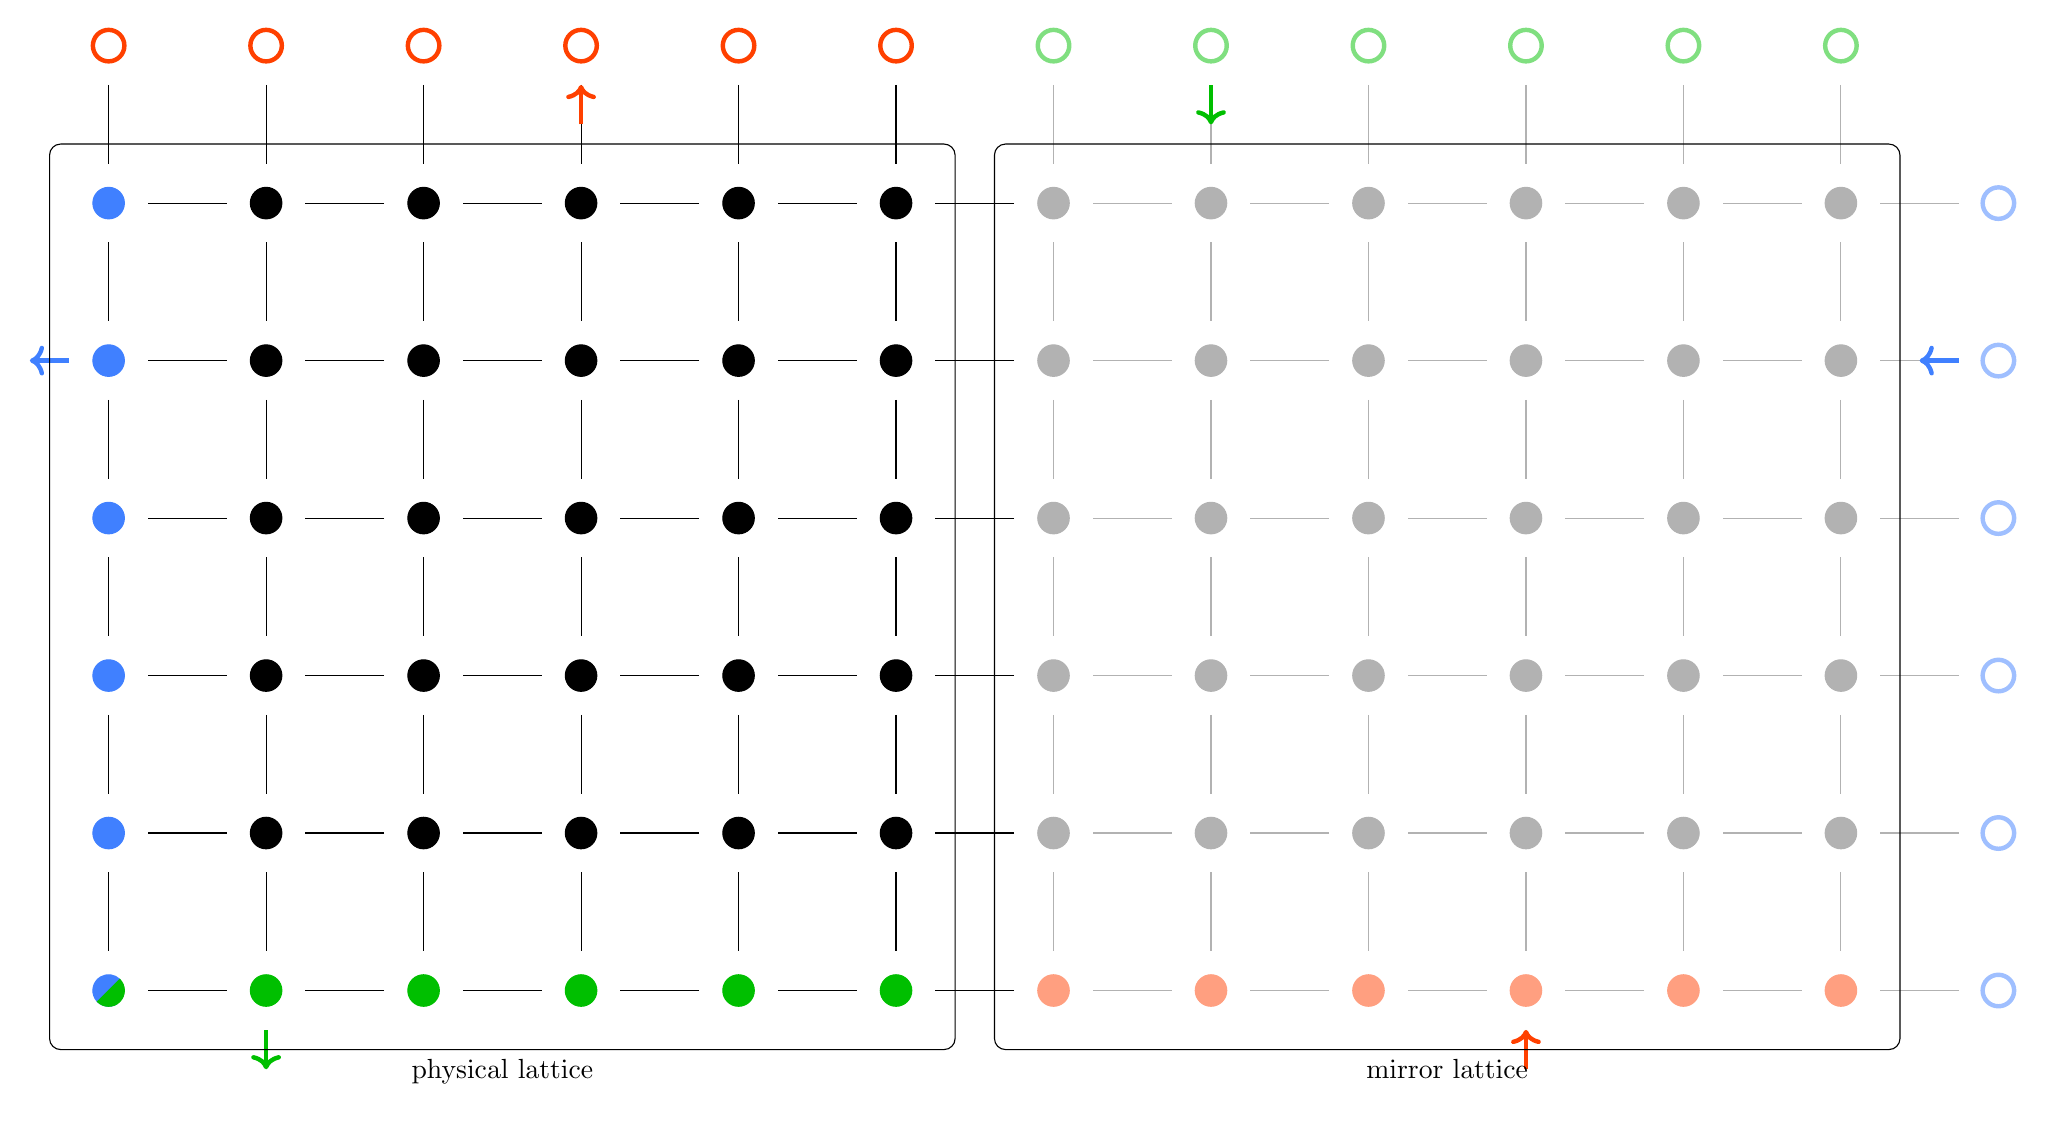
\begin{tikzpicture}
\foreach \x in {0,1,2,3,4,5,6,7,8,9,10,11,12} {
    \foreach \y in {0,1,2,3,4,5,6} {
        \coordinate (n) at ($\x*(20mm, 0)+\y*(0, 20mm)$);
        \coordinate (A1) at ($\x*(20mm, 0)+\y*(0, 20mm)+(0,15mm)$);
        \coordinate (B1) at ($\x*(20mm, 0)+\y*(0, 20mm)+(0,5mm)$);
        \coordinate (A2) at ($\x*(20mm, 0)+\y*(0, 20mm)+(15mm,0)$);
        \coordinate (B2) at ($\x*(20mm, 0)+\y*(0, 20mm)+(5mm,0)$);

        \ifthenelse{\x=12 \AND \y=6} {}{
            \ifthenelse{\x=12} {
                \draw[color=cblue!50,ultra thick](n) circle (0.2); % boundary
            } {};
            \ifthenelse{\y=6} {
                \ifthenelse{\x>5} {
                    \draw[color=cgreen!50,ultra thick](n) circle (0.2); % boundary
                }{
                    \draw[color=cred,ultra thick](n) circle (0.2); % boundary
                }
            } {};
        };

        \ifthenelse{\x=12 \OR \y=6} {} {
            \ifthenelse{\x>5} {
                \ifthenelse{\y=0} {
                    \filldraw[color=cred!50,fill=cred!50](n) circle (0.2); % mirror
                } {
                    \filldraw[color=black!30,fill=black!30](n) circle (0.2); % mirror
                }
                \draw[color=black!30] (A1) -- (B1);
                \draw[color=black!30] (A2) -- (B2);
            } {
                \ifthenelse{\x=0} {
                    \ifthenelse{\y=0} {
                        % origin point
                        \filldraw[color=cblue,fill=cblue] (n) -- (300:0.2) arc (300:45:0.2) -- cycle;
                        \filldraw[color=cgreen,fill=cgreen] (n) -- (0.2,0) arc[start angle=0, end angle=45,radius=0.2] -- (n);
                        \filldraw[color=cgreen,fill=cgreen] (n) -- (0.2,0) arc[start angle=0, end angle=-135,radius=0.2] -- (n);
                    }{
                        \filldraw[color=cblue,fill=cblue](n) circle (0.2); % physical
                    }
                }{
                    \ifthenelse{\y=0} {
                        \filldraw[color=cgreen,fill=cgreen](n) circle (0.2); % physical
                    } {
                        \filldraw[color=black,fill=black](n) circle (0.2); % physical
                    }
                };
                \draw (A1) -- (B1);
                \draw (A2) -- (B2);
            };
        };
    };
};

% green arrow
\coordinate (A) at ($1*(20mm, 0)+0*(0, 20mm)-(0,10mm)$);
\coordinate (B) at ($1*(20mm, 0)+0*(0, 20mm)-(0,5mm)$);
\draw[<-,color=cgreen,ultra thick] (A) -- (B);

\coordinate (A) at ($7*(20mm, 0)+6*(0, 20mm)-(0,10mm)$);
\coordinate (B) at ($7*(20mm, 0)+6*(0, 20mm)-(0,5mm)$);
\draw[<-,color=cgreen,ultra thick] (A) -- (B);

% blue arrow
\coordinate (A) at ($0*(20mm, 0)+4*(0, 20mm)-(10mm,0)$);
\coordinate (B) at ($0*(20mm, 0)+4*(0, 20mm)-(5mm,0)$);
\draw[<-,color=cblue,ultra thick] (A) -- (B);

\coordinate (A) at ($12*(20mm, 0)+4*(0, 20mm)-(10mm,0)$);
\coordinate (B) at ($12*(20mm, 0)+4*(0, 20mm)-(5mm,0)$);
\draw[<-,color=cblue,ultra thick] (A) -- (B);

% red arrow
\coordinate (A) at ($3*(20mm, 0)+6*(0, 20mm)-(0,10mm)$);
\coordinate (B) at ($3*(20mm, 0)+6*(0, 20mm)-(0,5mm)$);
\draw[->,color=cred,ultra thick] (A) -- (B);

\coordinate (A) at ($9*(20mm, 0)+0*(0, 20mm)-(0,10mm)$);
\coordinate (B) at ($9*(20mm, 0)+0*(0, 20mm)-(0,5mm)$);
\draw[->,color=cred,ultra thick] (A) -- (B);

% pyhsical and mirror rectangles
\draw[rounded corners] (-0.75,-0.75) rectangle +(11.5,11.5);
\draw[rounded corners] (11.25,-0.75) rectangle +(11.5,11.5); 

\node[below] at (5,-0.75){physical lattice};
\node[below] at (17,-0.75){mirror lattice};

\end{tikzpicture}

\end{document}